\chapter{Adversarial Anomaly Detection}\label{chap:aad}
In recent years, the use of Generative Adversarial Networks (GANs) has been explored in the context of anomaly detection. The main idea is to train a GAN to learn the distribution of the normal data and then use one or all modules to detect anomalies. This chapter presents the main concepts of GANs and how they can be used for anomaly detection in solar wind profiles. Additionally, every experiment that was undertaken with this purpose will be explained. The chapter is organized as follow:

\section{Generative Adversarial Networks}\label{sec:gan_background}
GANs were first introduced by \cite{goodfellow.etal_GenerativeAdversarialNets_} in their paper "Generative Adversarial Nets". Since then, many variations of GANs have surfaced and been applied to different areas like human face generation, image-to-image and text-to-image translation, and semantic generation, among others. The original GAN consisted of two models, a generator $G$ and a discriminator $D$. The task of the first model was to capture the distribution of the data and generate new examples from that distribution. The function of the discriminator $D$ is to distinguish actual samples from the fake data generated by $G$. The two components play an adversarial game in which $G$ tries to fool $D$ with increasingly realistic examples, and in turn, $G$ tries to detect the fake samples from $G$. The authors proposed an analogy that would help the problem's dynamics:

\noindent\textit{The generative model can be thought of as analogous to a team of counterfeiters trying to produce fake currency and use it without detection, while the discriminative model is analogous to the police trying to detect the counterfeit currency. Competition in this game drives both teams to improve their methods until the counterfeits are indistinguishable from the genuine articles.} (\cite{goodfellow.etal_GenerativeAdversarialNets_})

The problem is formulated as follows:
\begin{equation}
    \underset{G}{min}\ \underset{D}{max}\ V(D,G) = \mathbb{E}_{x \sim p_{data}(x)}[\log D(x)] + \mathbb{E}_{z \sim p_z(z)}[\log(1 - D(G(z))]
    \label{eq:gan_min_max}
 \end{equation}

 \noindent where $x$ represents the data, $z$ the latent space,  $p_{data}(x)$ is the distribution of the data and $p_z(z)$ is the distribution of the latent points (usually Gaussian) that $G$ uses to generate new samples. GANs can then be defined as a minimax game where $D$ tries to maximize $V$, as it tries to recognize generated and real images better; and, on the other hand, $G$ wants to minimize the function $V$ because its goal is to fool $G$ as many times as possible. 


\subsection{Common Challenges in the Training Phase}
Earlier GAN architectures were very unstable and hard to train. Despite some proposed solutions to these issues (\cite{radford.etal_UnsupervisedRepresentationLearning_2016,arjovsky.etal_WassersteinGenerativeAdversarial_}), GANs are still remarkably difficult to train. Following are some of the main problems experienced during this phase.\\

\noindent\textbf{Mode collapse.} Occurs when the GAN is incapable of reaching Nash equilibrium \footnote{Can be explained by the following analogy: Two players, Alice and Bob, chose strategies A and B; Alice has no other strategy to maximise her goal better, and Bob has no different strategy other than B to maximise his goal in response to Alice's choice (\url{https://en.wikipedia.org/wiki/Nash_equilibrium})} and is a consequence of poor generalisation. It can occur when the generator $G$ only creates samples from a subset of the data distribution or only learns part of the distribution. The leading causes for this issue can be attributed to a poor choice of the objective function (\cite{saxena.cao_GenerativeAdversarialNetworks_2022}). In other words, $G$ focuses on a small subset of samples that consistently fool the discriminator $D$.\\

\noindent\textbf{Vanishing gradients.} The discriminator $D$ does not provide enough information for $G$ to update its gradients \cite{little.etal_GenerativeAdversarialNetworks_2021}. $D$ can distinguish real samples from fake ones with high confidence, which in turn causes the loss function of $G$ to decrease towards 0. As $D$ gets better, the gradient of $G$ progressively decreases until virtually none of the layers are updated, and $G$ can't generate samples with new distributions. Some solutions for this problem include batch normalization and clipping.\\

\noindent\textbf{Evaluation metrics.} Due to their wide range of applications, no global evaluation function can be applied to every GAN. The evaluation function varies greatly from the context of the problem in which the GAN was used. In some instances, like image generation, the principal evaluation criteria are still done qualitatively (the outputs are analyzed by humans, who determine their quality). Evaluation functions are an essential part of machine learning and allow for the correct conclusions to be made \cite{saxena.cao_GenerativeAdversarialNetworks_2022}.

%\subsection{Established GAN architectures}\label{sec:other_gans}
% TODO Wasserstein, Conditional, Bidirectional

\subsection{Anomaly Detection with GANs}\label{sec:gan_anomaly_detection}

Several approaches can be employed when using GANs for anomaly detection. The most simple one is to train both $G$ and $D$ on the normal data distribution and then use the latter to classify new samples as normal or anomalous. This is not always possible as the discriminator only learns to distinguish between samples that come from the generator and real ones. There is no guarantee that the discriminator will be able to distinguish between normal and anomalous samples, as it might have only learned specific characteristics of $G$ that are not present in the anomalous samples.

To circumvent this issue, some studies \cite{ngo.etal_FenceGANBetter_2019, liu.etal_GenerativeAdversarialActive_2020} proposed changing the focus of the vanilla GAN to be more appropriate for anomaly detection tasks. Instead of learning the normal distribution $G$ is forced to only generate anomalous samples. By forcing $G$ to generate samples close, but not equal to the normal distribution, the discriminator $D$ will learn to distinguish between normal and anomalous samples. To accommodate this, small changes to the loss functions of $D$ and $G$ are made. The results are promising, but by altering the loss functions, the new implementations might have new issues that were not experienced in other implementations.

Other studies \cite{li.etal_MADGANMultivariateAnomaly_2019, zenati.etal_AdversariallyLearnedAnomaly_2018, bashar.nayak_TAnoGANTimeSeries_2020} have proposed employing $G$ as a way to detect anomalies. These approaches are usually based on the reconstruction error of $G$ to detect anomalies, which is calculated by measuring the distance of the current sample to its closest reconstruction created by $G$. Then, an anomaly detection score can be construed with this error, either alone or in combination with the classification of the discriminator. Defective samples will, in theory, have higher reconstruction errors and will be classified as anomalous by the discriminator, as both modules didn't learn to generate or classify them correctly.

More recently, the use of adversarial autoencoders (AAE) has been proposed \cite{zenati.etal_AdversariallyLearnedAnomaly_2018,wang.etal_AdVAESelfadversarialVariational_2020} to simultaneously encode/decode an input sample and constrain its latent space representation to a prior distribution. The encoder and decoder are trained simultaneously with the discriminator, which is trained to distinguish between the latent space distribution and the prior distribution. The encoder is then used to encode new samples to the learned latent space. The discriminator classifies the latent representation of the sample as being real or fake. Similar to all other approaches, the anomaly score can be calculated by using only the reconstruction error of the decoded sample, or by combining it with the classification of the discriminator.

These methods will be employed in the experiments of this thesis. The next section explains the different approaches used to detect anomalies in solar wind profiles with the help of adversarial learning.

\section{Experiments}\label{sec:gan_experiments}
\subsection{Anomaly Scores}\label{sec:gan_anomaly_scores}
In this section, the anomaly scores and methods are used throughout every experiment to detect anomalies in solar wind profiles. At the end of each experiment, the most suitable anomaly detection method was chosen based on the results.

The first, and simplest score is the classification of the discriminator, $D$. The values of the classification can range from 0 to 1, where values equal to 0 indicate a real sample and values closer to 1 indicate a fake label. The classification score is calculated by feeding the sample to the discriminator and obtaining the classification value. The classification score is calculated as follows:

\begin{equation}
    D_{s} = 1 - D(x)
\end{equation}

where $x$ represents a batch from the testing dataset.

The second score is the reconstruction error of the generator, $G$, and is based on the reconstruction technique of MAD-GAN \cite{li.etal_MADGANMultivariateAnomaly_2019}. The reconstruction process occurs iteratively for each ith batch, $x^i$ in the testing dataset. Like in the original method, the optimal latent representation for $x^i$ is obtained by first sampling a latent space variable, $Z^k$. Then, for a predefined set of iterations, $j$, the generator $G$ is used to generate a batch of reconstructions $G(Z^{k,j})$. Contrary to \cite{li.etal_MADGANMultivariateAnomaly_2019}, the distance between the original batch $x^i$ and the reconstructed batch $G(Z^{k,j})$ is calculated using the MSE loss function. In the next step, the residuals of the MSE functions are averaged and used to update the parameters of $Z^{k,j}$. After $j$ iterations the best reconstruction, $Z^{k,j}$, of $x^i$ is returned.

The reconstruction error is calculated directly with the MSE loss between the real batch and the reconstructed batch from the optimal latent representation, $Z^{k,j}$. The reconstruction error is calculated as follows:

\begin{equation}
    R_{err} = MSE(x^i, G(Z^{k,j}))
\end{equation}

The reconstruction process described above is in Algorithm \ref{alg:mse_reconstruction}.
\\

\noindent\makebox[\textwidth][c]{%
\begin{minipage}{0.7\linewidth}
    \begin{algorithm}[H]
        \caption{MSE Reconstruction}\label{alg:mse_reconstruction}
    \begin{algorithmic}
        \Input
            \Desc{$x^i$}{Input Batch}
            \Desc{$n$}{Number of iterations}
        \EndInput
        \Output
            \Desc{$Z^k$}{Optimal latent representation}
            \Desc{$R_{err}$}{MSE Reconstruction error}
        \EndOutput
    \end{algorithmic}

    \BlankLine
    \emph{Get a sample from the latent space}\;
    $Z^k = random\_sample()$\;
    \For{$j = 0$ \KwTo $n$}{
        \emph{Reconstruct batch from $Z^k$ and calculate loss}\;
        $R_{err} = MSE(x^i, G(Z^k))$\;
        \emph{Update latent representation based on $R_{err}$}\;
        $Z^k = update(Z^k, R_{err}$)\;
        }
    \end{algorithm}
\end{minipage}}

The next score is a combination of the previous two scores, as a way of taking advantage of both the discriminator and the generator in the detection process. The reconstruction process is similar to the previous one, but instead of using only the MSE loss, the classification score, $D_{s}$ of the discriminator is also used. The new altered loss function is defined as follows:

\begin{equation}
    RD_{err} = MSE(x^i, G(Z^{k,j})) + D_{s}
\end{equation}

The algorithm for the reconstruction process with the discriminator input is shown in Algorithm \ref{alg:mse_reconstruction}. It is very similar to Algo. \ref{alg:mse_reconstruction}, but with the addition of the discriminator classification score to the loss function.
\\

\noindent\makebox[\textwidth][c]{%
\begin{minipage}{0.7\linewidth}
    \begin{algorithm}[H]
        \caption{MSE-Discriminator Reconstruction}\label{alg:mse_discr_reconstruction}
        \begin{algorithmic}
            \Input
                \Desc{$x^i$}{Input Batch}
                \Desc{$n$}{Number of iterations}
            \EndInput
            \Output
                \Desc{$Z^k$}{Optimal latent representation}
                \Desc{$RD_{err}$}{MSE-Discr. Reconstruction error}
            \EndOutput
        \end{algorithmic}
        
        \BlankLine
        \emph{Get a sample from the latent space}\;
        $Z^k = random\_sample()$\;
        \For{$j = 0$ \KwTo $n$}{
            \emph{Obtain $D$ classification for reconstructed batch}\;
            $D_s = 1 - D(G(Z^k))$\;

            \emph{Reconstruct batch from $Z^k$ and calculate loss}\;
            $RD_{err} = MSE(x^i, G(Z^k)) \times D_s$\;
            \emph{Update latent representation based on $RD_{err}$}\;
            $Z^k = update(Z^k, RD_{err}$)\;
        }
    \end{algorithm}
\end{minipage}}

\section{Linear GAN}\label{sec:gan_experiment_1}

\begin{figure}
    \centering
    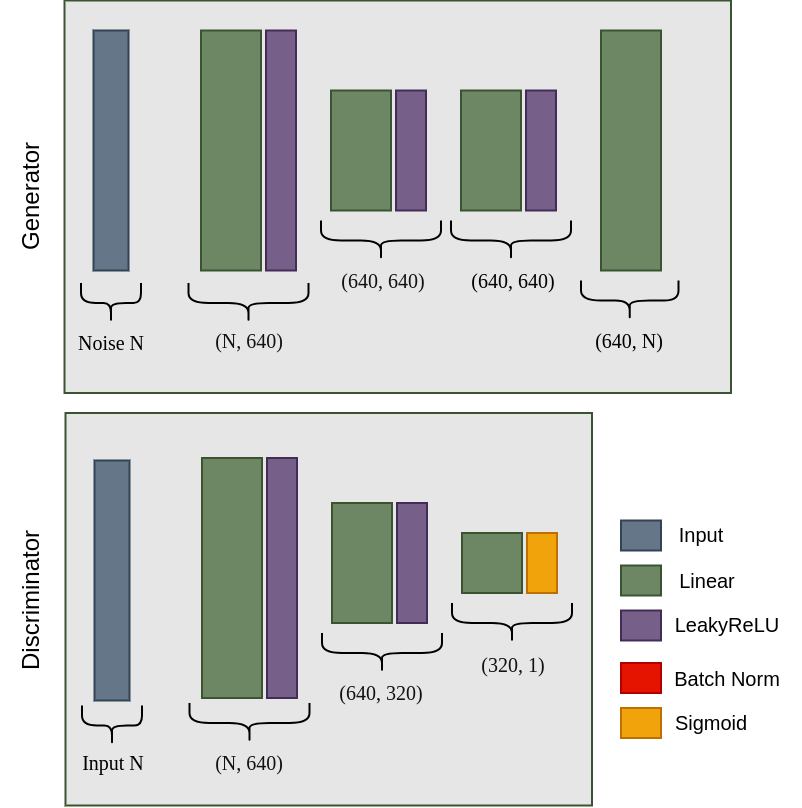
\includegraphics[width=0.8\textwidth]{figures/linearGAN.png}
    \caption{Linear GAN Architecture}
    \label{fig:linear_gan_architecture}
\end{figure}


The first architecture was a linear GAN, which is a simple GAN with a linear generator and discriminator. Several experiments were performed with different configurations of the architecture. The use of BatchNorm in either module was tested, to try and stabilize the training process. This proved to be ineffective as it made it difficult for $G$ and $D$ to converge. Because of this, it was not included in the final implementation. In addition to this, the number of intermediate stacked linear layers was varied during the tests to try and find a configuration that worked best for this problem. 

Besides these changes, different activation functions were also tested. The activation functions used were ReLU, LeakyReLU, and Tanh, with a combination of them in the intermediate as well as in the output and input layers. Similar to other GAN architectures, the LeakyReLU activation function was chosen to prevent the gradient from vanishing, and to improve the overall stability of the learning process. Most configurations that included the Tanh activation function in the output layer of the generator were discarded, as it proved to not be effective during the anomaly detection phase.

The final architecture is shown in Fig. \ref{fig:linear_gan_architecture}. Both the generator and discriminator are built with linear layers. The generator, $G$, consists of an input layer that takes as input a latent space variable, $Z$ with size $N$, and outputs a sample with the same dimension as the input. The first layer performs a linear transformation on the input noise vector and projects $Z$ into lower dimensional space with 640 dimensions. The output of this layer is then passed through a LeakyReLU activation function. Next, the resulting features from this step are passed through two stacked linear layers, each with 630 dimensions. In the last layer, the features from the previous step undergo a linear transformation to project them into the same dimension as the input sample. As was previously said, no activation function is used in the output layer of the generator, because it proved to not be effective during the detection phase.

The discriminator, $D$, consists of an input layer that takes as input a sample with $N$ features and outputs a scalar value. The objective of $D$ is to progressively learn the most important features of the data to perform binary classification of the input sample as being real or fake. The first and subsequent layers perform linear transformations of the input data into increasingly smaller dimensions. In the output layer, the features from the previous step are projected into a single scalar value. This value is then passed through a sigmoid activation function to obtain the final classification score of each sample.

Both modules were trained with the Adam optimizer with a learning rate of 0.0001 for the generator and 0.0002 for the discriminator. This was done to prevent the discriminator from overpowering the generator during the training process. The weights of each of the linear layers were initialized with the He initialization function from \cite{He.Zhang.ea_DelvingDeepRectifiers_2015}.

Two models were trained, one to detect anomalies in the inputs of the MULTI-VP dataset and the other in the outputs (refer to Chapter \ref{chap:eda}). Both models were trained over 300 epochs with a batch size of 128. In both approaches the training data was scaled with the \textit{MinMaxScaler} to preserve the variation of extreme values in the data. The training data consisted of a matrix with $M\times N$ dimension, where $M$ is the number of training samples and $N$ is the number of features per sample. The same validation files from the clustering experiments were excluded from the training process in both approaches.

In the first model, the input data, $X_i$, consists of the concatenation of the $B [G]$ and $\alpha [deg]$ input variables for each profile. The radial coordinate radius, $R [R_{sun}]$ was excluded from the process, to reduce the number of features the networks needed to learn. In addition to this, extreme variations in the input data were removed to prevent both modules from learning noisy features that would hinder the detection process. The number of features, $N_i$, for each of the input samples is 1280.

In the outputs model, every output variable of MULTI-VP is used in the training phase. Each sample consists of the concatenation of the density, $n [10^{10}cm^{-3}]$,  the velocity, $v [km/s]$, and temperature, $T [MK]$, with a combined number of features per sample, $N_o$, of 1920. Contrary to the input model, no extreme variations were removed from the data, as it performed well without this step.

The detection step was carried out for each of the models with all three anomaly score functions of Sec. \ref{sec:gan_anomaly_scores}. Due to the lack of validation metrics, the choice of method was based on the visual inspection of the results. The stability of the anomaly scores as well as the quality of the dataset without anomalies were taken into account.

Having these factors into consideration, the best results were obtained with the reconstruction error, $R_{err}$. The other two functions, $D_{err}$ and $D_{err} + RD_{err}$, were very unstable and were not able to detect the anomalies as well as $R_{err}$. The filtered input and output variables can be seen in Image \ref{fig:linear_gan_clean_in} and \ref{fig:linear_gan_clean_out} respectively.


\begin{figure}[]
    \caption[Linear GAN filtered datasets]{Resulting datasets after the anomaly detection step with the linear GAN architecture on the inputs and outputs of the MULTI-VP dataset.}
    \label{fig:linear_gan_clean_data}
    \begin{subfigure}[h]{0.6\textwidth}
        \centering
        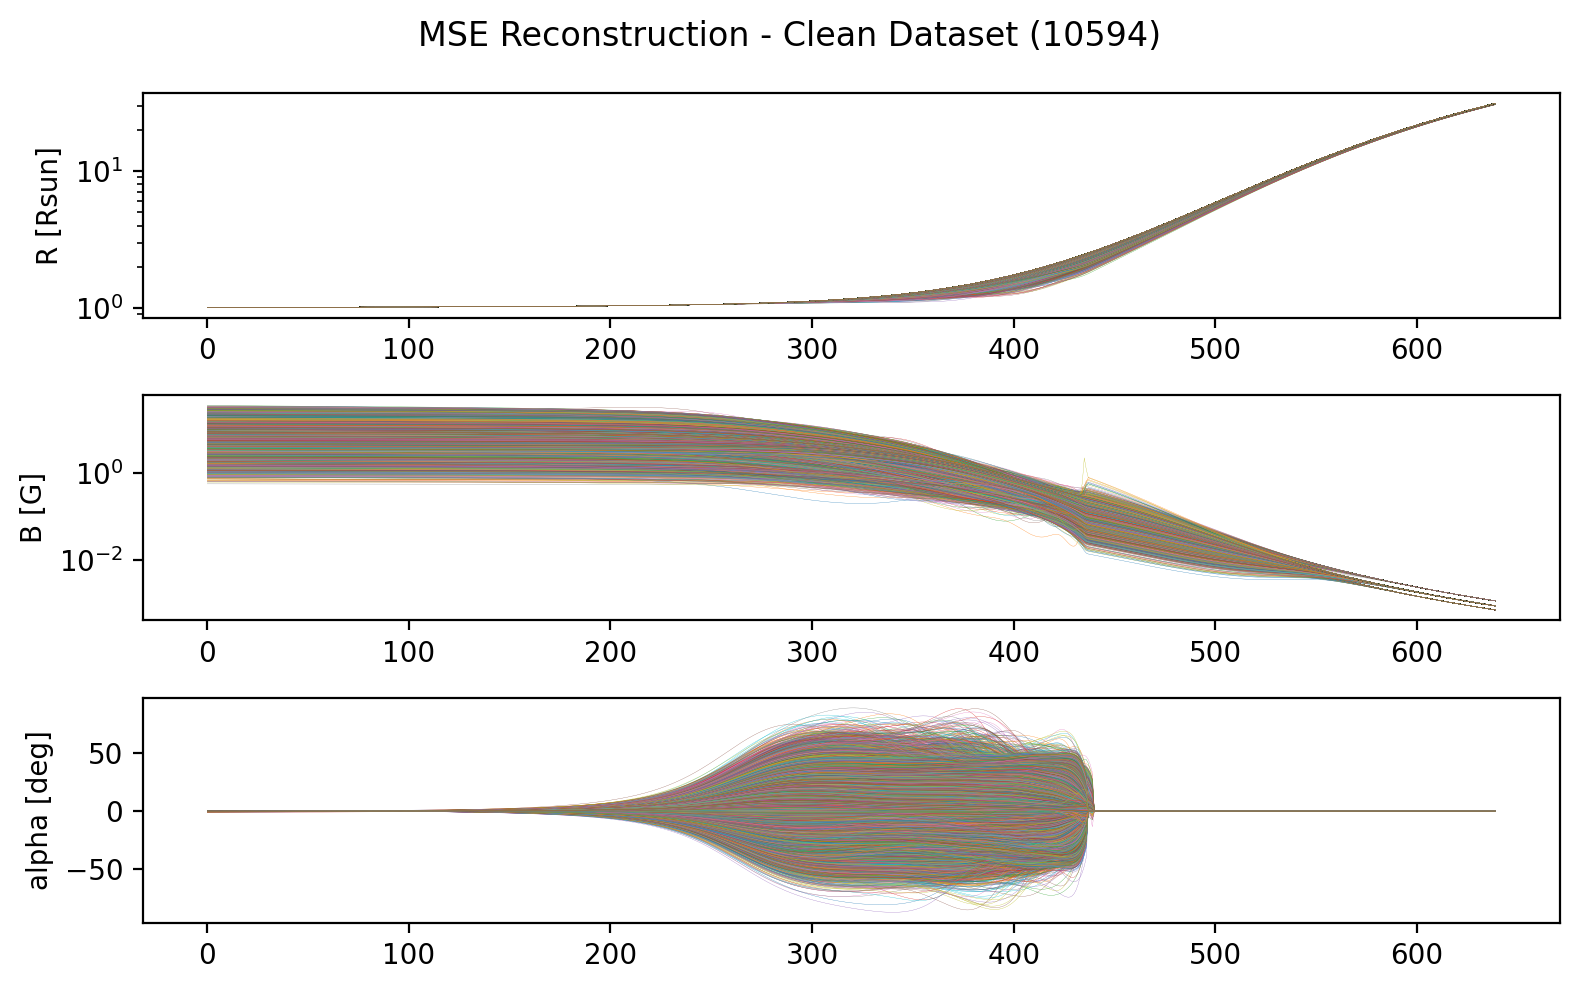
\includegraphics[width=\textwidth]{figures/linearGAN_clean_in.png}
        \caption{Input Variables}
        \label{fig:linear_gan_clean_in}
        % \label{fig:tsne_mag_2d}
    \end{subfigure}
    \hfill
    \begin{subfigure}[h]{0.6\textwidth}
        \centering
        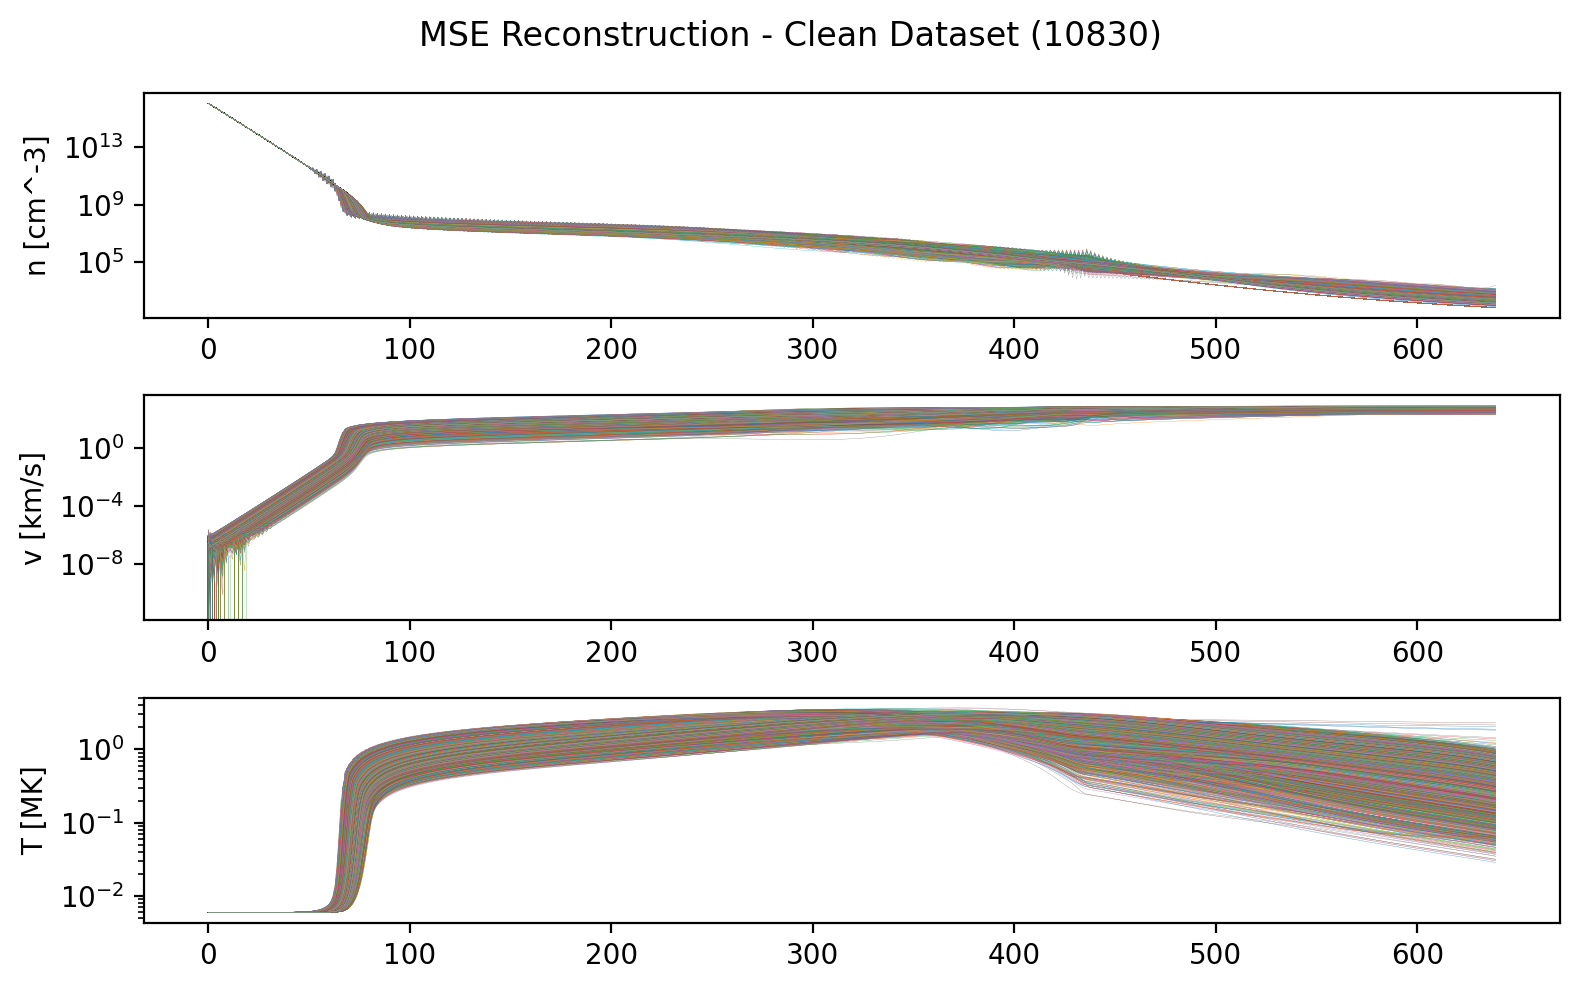
\includegraphics[width=\textwidth]{figures/linearGAN_clean_out.png}
        \caption{Output Variables}
        \label{fig:linear_gan_clean_out}
    \end{subfigure}
\end{figure}

The first image (Fig. \ref{fig:linear_gan_clean_in}) resulted from removing 10\% of the files from the original dataset based on anomaly scores. As was previously said, the anomaly scores were obtained by training the GAN model in the input variables and then using the $G$ to calculate the noamly scores oof each sample in the testing dataset. The results show that the data is moslty clean, with some anomalies still remaining in the magnetic field, $B [G]$, variable.

For the output variables (Fig. \ref{fig:linear_gan_clean_out}) only 8\% of the files were excluded based on anomaly scores. The resulting output variables are mostly clean, with some abnormalities in the density, $n [cm^3]$, variable.

Overall, the experiments with this architecture prove that it can detect anomalies in the input and output variables of MULTI-VP. However, the percentage of files that need to be removed (i.e. the False Positive rate) is still very high. This might indicate that the current architecture might not be the most ideal for the task, as seamingly "normal" profiles might be excluded from the prediction step.










\section{Experiment 2: LSTM-RNN GAN}\label{sec:gan_experiment_2}
\section{Experiment 4: VAE}\label{sec:mad-gan}
\section{Experiment 3: AAE}\label{sec:gan_experiment_3}

